%% Compétences : 6C05-NUM09, 6C05-NUM10, 6C05-NUM11, 6C05-NUM12, 6C05-NUM13, 6C05-NUM14
%% Cours (trace écrite copiée au tableau) : une partie par compétence.

%% Font size %%
\documentclass[11pt]{article}

%% Load the custom package
\usepackage{Mathdoc}
\usepackage{icomma}
\usepackage{colortbl}
\usetikzlibrary{decorations.pathreplacing}

%% Numéro de séquence %% Titre de la séquence %%
\renewcommand{\centerhead}{S05 - Les nombres décimaux}

% Encadré « compétence » en tête de partie
\newcommand{\comp}[2]{\par\smallskip\noindent\colorbox{gray!15}{\parbox{\dimexpr\linewidth-2\fboxsep}{\small\textbf{Compétence #1} : #2}}\par\smallskip}
% Fraction lisible en ligne
\newcommand{\f}[2]{\dfrac{#1}{#2}}

% Version élève (VE) : Cours-6C05-Nombres-Decimaux-VE.tex fait \def\versioneleve{} puis \input ce fichier.
% Version prof (ce fichier seul) : réponses en rouge = corrigé des parties à compléter.
\newif\ifve \ifdefined\versioneleve\vetrue\fi
\ifve\renewcommand{\centerhead}{S05 - Les nombres décimaux (élève)}\fi
% Réponse : en rouge (prof), vide de même largeur (élève)
\newcommand{\rep}[1]{\ifve\phantom{#1}\else\textcolor{red}{#1}\fi}
% Réponse sur pointillés de largeur #1 (élève)
\newcommand{\pts}[2][3cm]{\ifve\makebox[#1]{\dotfill}\else\textcolor{red}{#2}\fi}
% Définition à écrire : #1 lignes de pointillés espacées (élève), texte (prof)
\newcommand{\lignes}[2]{\ifve\par\foreach \k in {1,...,#1}{\vspace{8mm}\noindent\makebox[\linewidth]{\dotfill}\par}\else #2\fi}
% Chiffre du tableau de numération : gros ; \chg = exemple traité (gris)
\newcommand{\chg}[1]{\Large\textcolor{gray}{\textbf{#1}}}
\newcommand{\ch}[1]{\Large #1}
\newcommand{\chr}[1]{\Large\rep{#1}}

%% Spacing commands %%
\renewcommand{\baselinestretch}{1} \setlength{\parindent}{0pt}

\begin{document}

% Version élève : seulement les parties II et IV, une page recto chacune (collées dans le cahier).
\ifve\else
\begin{tcolorbox}[colback=white,colframe=black,boxrule=0.6pt,arc=2mm,title={\textbf{Ce que je dois savoir faire à la fin du chapitre}},coltitle=black,colbacktitle=gray!15]
\begin{tabular}{@{}ll@{}}
\textbf{6C05-NUM09} & Reconnaître une \textbf{fraction décimale} \hfill (partie 1)\\
\textbf{6C05-NUM10} & \textbf{Lire et écrire} un nombre décimal \hfill (partie 2)\\
\textbf{6C05-NUM11} & \textbf{Décomposer} un nombre décimal \hfill (partie 3)\\
\textbf{6C05-NUM12} & Placer un décimal sur une \textbf{demi-droite graduée} \hfill (partie 4)\\
\textbf{6C05-NUM13} & \textbf{Comparer} et \textbf{encadrer} des décimaux \hfill (partie 5)\\
\textbf{6C05-NUM14} & Donner une \textbf{valeur approchée} ou un \textbf{arrondi} \hfill (partie 6)\\
\end{tabular}
\end{tcolorbox}

%% ------------------------------------------------------------------
\section{Les fractions décimales}
\comp{6C05-NUM09}{reconnaître une fraction décimale \hfill \textit{Fiche Ex-6C05-01}}

\begin{definition}
Une \textbf{fraction décimale} est une fraction dont le dénominateur est $10$, $100$, $1\,000$\ldots
\end{definition}

\begin{center}
\renewcommand{\arraystretch}{1.6}
\begin{tabular}{|c|c|c|}
\hline
$\f{1}{10} = 0,1$ & $\f{1}{100} = 0,01$ & $\f{1}{1\,000} = 0,001$ \\
\textbf{un dixième} & \textbf{un centième} & \textbf{un millième} \\ \hline
\end{tabular}
\qquad
\begin{tabular}{l}
$1$ unité $= 10$ dixièmes\\
$1$ dixième $= 10$ centièmes\\
$1$ centième $= 10$ millièmes
\end{tabular}
\end{center}

\begin{exemple}
$\f{7}{10}$ se lit « sept dixièmes » ; \quad $\f{34}{100}$ se lit « trente-quatre centièmes » ; \quad
$\f{3}{4}$ \textbf{n'est pas} une fraction décimale.
\end{exemple}

\fi
%% ------------------------------------------------------------------
\ifve\setcounter{section}{1}\fi
\section{L'écriture à virgule}
\comp{6C05-NUM10}{lire et écrire un nombre décimal \hfill \textit{Fiche Ex-6C05-02}}

\begin{definition}
\lignes{3}{Un \textbf{nombre décimal} peut s'écrire avec une \textbf{virgule}. La virgule sépare la
\textbf{partie entière} (à gauche) de la \textbf{partie décimale} (à droite).}
\end{definition}

\noindent\begin{minipage}{\linewidth}
\begin{exemple}[Je place le nombre dans le tableau de numération]
Je place chaque nombre dans le tableau, puis j'écris son écriture à virgule. \textit{La première ligne est faite (en gris).}
\end{exemple}

\begin{center}
\renewcommand{\arraystretch}{2.1}
\setlength{\tabcolsep}{3.5pt}
\begin{tabular}{|>{\raggedright\arraybackslash}m{5.4cm}|*{3}{>{\centering\arraybackslash}m{6mm}|}*{3}{>{\centering\arraybackslash}m{6mm}|}>{\centering\arraybackslash}m{2mm}|*{3}{>{\centering\arraybackslash}m{9mm}|}>{\centering\arraybackslash}m{2.6cm}|}
\hline
\multicolumn{1}{|c|}{\textbf{Nombre}} & \multicolumn{3}{c|}{\small\textbf{Milliers}} & \multicolumn{3}{c|}{\small\textbf{Unités}} & & \multicolumn{3}{c|}{\small\textbf{Partie décimale}} & \textbf{Écriture} \\
\multicolumn{1}{|c|}{} & \small C & \small D & \small U & \small C & \small D & \small U & & $\f{1}{10}$ & $\f{1}{100}$ & $\f{1}{1000}$ & \textbf{à virgule} \\ \hline
\textcolor{gray}{\small\textit{Exemple :} trente-deux unités et quarante-cinq centièmes} & & & & & \chg{3} & \chg{2} & \textbf{,} & \chg{4} & \chg{5} & & \textcolor{gray}{\Large$\mathbf{32,45}$} \\ \hline\hline
$35,7$ & & & & & \chr{3} & \chr{5} & \textbf{,} & \chr{7} & & & $35,7$ \\ \hline
$\f{408}{100}$ & & & & & & \chr{4} & \textbf{,} & \chr{0} & \chr{8} & & \rep{$4,08$} \\ \hline
\small douze unités et cinq centièmes & & & & & \chr{1} & \chr{2} & \textbf{,} & \chr{0} & \chr{5} & & \rep{$12,05$} \\ \hline
$0,903$ & & & & & & \chr{0} & \textbf{,} & \chr{9} & \chr{0} & \chr{3} & $0,903$ \\ \hline
$\f{12\,504}{10}$ & & & \chr{1} & \chr{2} & \chr{5} & \chr{0} & \textbf{,} & \chr{4} & & & \rep{$1\,250,4$} \\ \hline
\small trois-cents unités et sept millièmes & & & & \chr{3} & \chr{0} & \chr{0} & \textbf{,} & \chr{0} & \chr{0} & \chr{7} & \rep{$300,007$} \\ \hline
\end{tabular}
\end{center}
\end{minipage}
\medskip


\begin{exemple}[Je lis un nombre décimal]
$32,45$ : la partie entière est $32$, la partie décimale est $0,45$.
On lit : « trente-deux \textbf{unités} et quarante-cinq \textbf{centièmes} »
ou « trente-deux \textbf{virgule} quarante-cinq ».

\renewcommand{\arraystretch}{2}
\begin{tabular}{@{}l@{\;}l@{}}
$35,7$ se lit : & \pts[13cm]{trente-cinq unités et sept dixièmes} \\
$0,903$ se lit : & \pts[13cm]{zéro unité et neuf-cent-trois millièmes} \\
$4,08$ : partie entière \pts[2cm]{$4$}, & partie décimale \pts[2cm]{$0,08$} \\
\end{tabular}
\end{exemple}

\ifve\else
\begin{remarque}
\textbf{Les zéros inutiles} : on peut ajouter ou enlever des zéros \textbf{à droite de la partie décimale}
ou \textbf{à gauche de la partie entière} sans changer le nombre :
$\quad 05,30 = 5,3 \qquad 12 = 12,0 = 12,00$.\\
\textbf{Attention :} $5,03 \neq 5,3$ \quad (ce zéro est utile : il dit qu'il y a $0$ dixième).
\end{remarque}
\fi

\ifve\newpage\else
%% ------------------------------------------------------------------
\section{Décomposer un nombre décimal}
\comp{6C05-NUM11}{décomposer un nombre décimal \hfill \textit{Fiche Ex-6C05-03}}

\begin{exemple}[Chiffre des\ldots]
Dans $562,708$ : le chiffre des \textbf{dizaines} est $6$, le chiffre des \textbf{dixièmes} est $7$,
le chiffre des \textbf{centièmes} est $0$, le chiffre des \textbf{millièmes} est $8$.
\end{exemple}

\begin{propriete}
Un nombre décimal peut s'écrire de plusieurs façons :
\[
562,708 \;=\; 500 + 60 + 2 + \f{7}{10} + \f{0}{100} + \f{8}{1\,000}
\;=\; 562 + \f{708}{1\,000}
\;=\; \f{562\,708}{1\,000}
\]
\end{propriete}

\begin{remarque}
Le nombre de chiffres après la virgule donne le dénominateur :
$1$ chiffre $\to 10$, \quad $2$ chiffres $\to 100$, \quad $3$ chiffres $\to 1\,000$.
\qquad Ex. : $4,06 = \f{406}{100}$.
\end{remarque}

\fi
%% ------------------------------------------------------------------
\ifve\setcounter{section}{3}\fi
\section{Repérer un nombre sur une demi-droite graduée}
\comp{6C05-NUM12}{placer un décimal sur une demi-droite graduée \hfill \textit{Fiches Ex-6C05-04 et 05}}

\begin{definition}
\lignes{3}{Une \textbf{demi-droite graduée} a une \textbf{origine} (le point d'abscisse $0$) et une
\textbf{unité} reportée régulièrement. Un point est repéré par un nombre : son \textbf{abscisse}.}
\end{definition}

\begin{remarque}
Pour lire une graduation, je cherche d'abord \textbf{combien vaut un petit intervalle} :
ici l'unité est partagée en $10$, donc un petit intervalle vaut $0,1$ (un dixième).
\end{remarque}

\begin{exemple}[Lire une abscisse]
L'abscisse du point $A$ est $2,4$ : on écrit $A(2,4)$. \quad Je lis l'abscisse des autres points.

\begin{center}
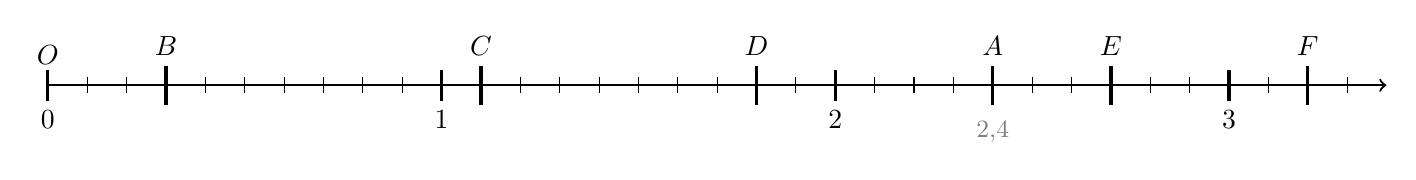
\begin{tikzpicture}[x=5cm,y=1cm]
  \draw[->,thick] (0,0) -- (3.4,0);
  \foreach \i in {0,...,33} \draw (\i*0.1,-0.1) -- (\i*0.1,0.1);
  \foreach \i in {0,1,2,3} {\draw[very thick] (\i,-0.2) -- (\i,0.2); \node[below] at (\i,-0.2) {$\i$};}
  \node[above=4pt] at (0,0) {$O$};
  \foreach \x/\n in {2.4/A,0.3/B,1.1/C,1.8/D,2.7/E,3.2/F}
    {\draw[very thick] (\x,-0.25) -- (\x,0.25); \node[above] at (\x,0.25) {$\n$};}
  \node[below=4pt,gray] at (2.4,-0.2) {\small $2,4$};
\end{tikzpicture}

\renewcommand{\arraystretch}{2.2}
\begin{tabular}{*{3}{l@{\hspace{1.2cm}}}}
\textcolor{gray}{$A(2,4)$} & $B$( \pts[1.8cm]{$0,3$} ) & $C$( \pts[1.8cm]{$1,1$} ) \\
$D$( \pts[1.8cm]{$1,8$} ) & $E$( \pts[1.8cm]{$2,7$} ) & $F$( \pts[1.8cm]{$3,2$} ) \\
\end{tabular}
\end{center}
\end{exemple}

\begin{exemple}[Placer un point]
Le point $M(5,3)$ est placé. \quad Je place les points $N(5,8)$ \quad $P(6,1)$ \quad $R(6,5)$ \quad $S(6,9)$ \quad $T(5,05)$.

\begin{center}
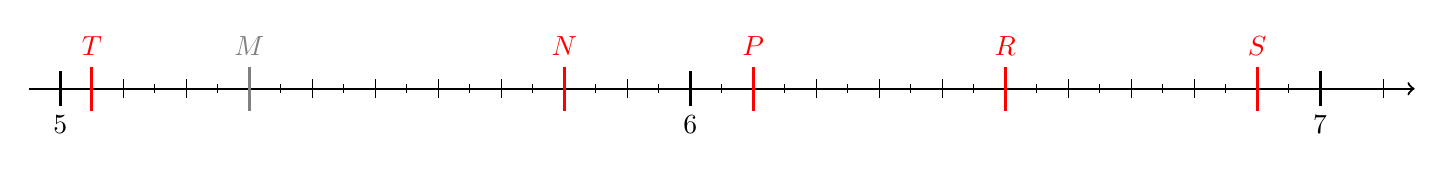
\begin{tikzpicture}[x=8cm,y=1cm]
  \draw[->,thick] (4.95,0) -- (7.15,0);
  \foreach \i in {0,...,40} \draw (5+\i*0.05,-0.06) -- (5+\i*0.05,0.06);
  \foreach \i in {0,...,21} \draw (5+\i*0.1,-0.12) -- (5+\i*0.1,0.12);
  \foreach \i in {5,6,7} {\draw[very thick] (\i,-0.22) -- (\i,0.22); \node[below] at (\i,-0.22) {$\i$};}
  \draw[very thick,gray] (5.3,-0.28) -- (5.3,0.28) node[above] {$M$};
  \ifve\else
  \foreach \x/\n in {5.8/N,6.1/P,6.5/R,6.9/S,5.05/T}
    {\draw[very thick,red] (\x,-0.28) -- (\x,0.28) node[above] {$\n$};}
  \fi
\end{tikzpicture}
\end{center}
\textit{Ici, entre deux dixièmes, il y a un trait de plus : il marque les demi-dixièmes ($0,05$).}
\end{exemple}

\ifve\else
%% ------------------------------------------------------------------
\section{Comparer, ranger et encadrer}
\comp{6C05-NUM13}{comparer et encadrer des décimaux \hfill \textit{Fiche Ex-6C05-06}}

\begin{propriete}[Comparer deux décimaux]
\begin{enumerate}
\item On compare d'abord les \textbf{parties entières} : $12,9 < 13,1$ car $12 < 13$.
\item Si elles sont égales, on compare chiffre à chiffre : les \textbf{dixièmes}, puis les \textbf{centièmes}\ldots
\end{enumerate}
\end{propriete}

\begin{exemple}
Comparer $4,7$ et $4,65$ : même partie entière $4$ ; dixièmes : $7 > 6$ ; donc $4,7 > 4,65$.\\
\textit{Astuce :} on ajoute des zéros inutiles pour avoir autant de chiffres : $4,70 > 4,65$.
\end{exemple}

\begin{vocabulaire}
\textbf{Ranger dans l'ordre croissant} : du plus petit au plus grand ($<$).
\textbf{Ordre décroissant} : du plus grand au plus petit ($>$).\\
\textbf{Encadrer} un nombre, c'est l'écrire entre deux nombres :
$\;7 < 7,38 < 8$ \;(à l'unité), \quad $7,3 < 7,38 < 7,4$ \;(au dixième).
\end{vocabulaire}

%% ------------------------------------------------------------------
\section{Valeur approchée et arrondi}
\comp{6C05-NUM14}{donner une valeur approchée ou un arrondi \hfill \textit{Fiches Ex-6C05-07 et 08}}

\begin{definition}
Dans l'encadrement $7,3 < 7,38 < 7,4$ :
$7,3$ est la valeur approchée \textbf{par défaut} au dixième, $7,4$ la valeur approchée \textbf{par excès}.\\
L'\textbf{arrondi} est la valeur approchée la \textbf{plus proche} du nombre.
\end{definition}

\begin{propriete}[Arrondir]
On regarde le chiffre \textbf{juste après} le rang demandé :
s'il vaut $0$, $1$, $2$, $3$ ou $4$, on garde ; s'il vaut $5$, $6$, $7$, $8$ ou $9$, on \textbf{augmente} de $1$.
\end{propriete}

\begin{exemple}
Arrondi de $7,38$ au dixième : le chiffre après les dixièmes est $8$, donc $7,38 \approx 7,4$.\\
Arrondi de $15,62$ à l'unité : le chiffre des dixièmes est $6$, donc $15,62 \approx 16$.
\end{exemple}

\fi
\end{document}

%%% Local Variables:
%%% mode: LaTeX
%%% TeX-master: t
%%% End:
